\section{Unfolding the matrix power} 
\label{sec:appendix-unfold}
In this part of the appendix, we define formally the unfolding function
\begin{align*}
    \ranked{\tmonad \mati k{\Sigma} \to \mati k{( \tmonad \Sigma)}}
\end{align*}
that was described in Section~\ref{sec:unfolding}. We  present the definition in a slightly verbose manner,  by  decomposing unfolding into simpler operations. The  presentation highlights the inductive character of unfolding, and the reasons why we are uneasy about it being a prime operation. 
%  The simpler operations  will be used in Appendix~\ref{ap:matrix-power}, where we show how to derive the (monotone) unfolding operation.



\subsection{Shallow terms}
\label{sec:shallow-terms}
We begin by defining unfolding  for terms of depth two, called \emph{shallow terms}. Later, we extend the definition to all other terms by induction. 
We describe shallow terms as a separate datatype, since this datatype will also be used later, in Section~\ref{ap:matrix-power}, to derive the (monotone) unfolding operation.
 For now, shallow terms are just an intermediate type used to define formally the unfolding function. 

 Let $\rSigma$ and $\rGamma$ be two ranked sets. The  shallow terms datatype, which is  denoted $\shallowterm \rSigma \rGamma$, consists of  expressions of the form $a\tensorpair{b_1,\dots,b_n}$ where $a$ is an $n$-ary element of $\rSigma$ and $b_1,\dots, b_n$ are elements of $\rGamma$. The arity of such an expression is the sum of arities of $b_1,\ldots,b_n$. We draw shallow terms as terms of depth two, where the root is from $\rSigma$ and  the children are from $\rGamma$:
\mypic{54}
An equivalent definition of shallow terms, in terms of products and co-products, is 
\begin{align}\label{eq:shallowterm-definition}
\shallowterm \rSigma \rGamma \quad \eqdef   \quad \ranked{\coprod_{\black{a \in} \rSigma} } \overbrace{\ranked{\Gamma \product \cdots \product \Gamma},}^{\text{arity of $a$ times}}
\end{align}


\subsection{Terms as an inductive datatype}
\label{sec:terms-induction-principle}
Using shallow terms, we can define the set of terms as the least solution of the equation
\begin{align*}
\ranked{\tmonad \rSigma = \set{\portletter} + \shallowterm \Sigma {(\tmonad \rSigma)}}.
\end{align*}
With this inductive definition, in order to define an operation of type $\ranked{ \tmonad \rSigma \to \Gamma}$
on terms, it is enough to explain the induction base for the  identity term and the induction step for shallow unfolding, as captured by two operations of types
\begin{align*}
        \underbrace{\ranked{\set \portletter \to \Gamma}}_{\text{induction base}}
        \qquad 
        \underbrace{\ranked{\shallowterm \Sigma \Gamma \to \Gamma}.}_{\text{induction step}}
\end{align*}
We use such an induction below to define general unfolding.  The crucial step is defining the induction step, which the unfolding for shallow terms defined in Section~\ref{sec:definition-of-shallow-unfolding} below. 

 As mentioned at the beginning of Section~\ref{sec:derivable-functions}, the guiding principle behind our approach is to avoid iteration mechanisms. The inductive definition of general unfolding could be seen as such an iteration mechanism; this is the reason for Section~\ref{ap:matrix-power}, where (monotone) unfolding is derived using simpler operations.  In contrast, we believe that iteration is indeed avoided by  the operations used in the induction step that are presented in Section~\ref{sec:definition-of-shallow-unfolding} below.

We do not formalise what we mean by  ``avoiding iteration''. One possible direction would be to say that an operation ``avoids iteration'' if it can be computed by a family of bounded depth circuits, as in the circuit class AC$^0$. A further requirement could be that the family of circuits not only exists, but it is also easy to see. 

\subsection{Unfolding for shallow terms} 
\label{sec:definition-of-shallow-unfolding}
The induction step in general unfolding is the operation
\begin{align*}
    \ranked{
        \xymatrix{
            \shallowterm{\mati k \rSigma} {\mati k \rGamma}  \ar[r] & \mati k {(\shallowterm \Sigma \Gamma)},
        }
    }
\end{align*}
which we call shallow unfolding, and   
which is explained in the following picture:
\mypic{121}
To define this operation formally, we further decompose it using  three functions manipulating shallow terms. These functions, which are used here as  intermediate functions in the definition of shallow unfolding, will become prime functions when we decompose the unfolding function in Appendix~\ref{ap:matrix-power}.

\subsubsection{Distribute shallow terms over fold}
 Let $\rGamma$ and $\rSigma$ be two datatypes.  Consider the function $\ranked{f_1}$
\begin{align*}
\ranked{\shallowterm  \Gamma {\reduce k \Sigma}} \ranked{\xrightarrow{\quad f_1 \quad}} \ranked{\reduce k(\shallowterm  \Gamma  \Sigma)}
\end{align*}
which distributes shallow terms over folding. This function is illustrated by the following picture
\mypic{55}
and  defined by 
$$\begin{array}{rcl} 
a(b_1/g_1,\dots,b_n/g_n)&\mapsto& a(b_1,\dots,b_n)/g
\end{array}$$
where $g$ is the function defined as follows. For every  $i \in\set{1,\dots,n}$,  if  $j\in\set{1,\dots,\arity{b_i}}$ then 
 \begin{align*}
 \xymatrix@C=5cm{
 \begin{array}{c}
 \overbrace{j+\underset{l<i}{\Sigma} \arity{b_l}}^{\text{Position of the $j$-th port of $b_i$ is shifted}}
 \end{array}
 \ar@{|->}[d]^{g}\\
 \begin{array}{c}
  \biggl(\ \ \ \underbrace{\pi_2(g_i(j))+\underset{l<i}{\Sigma} \arity{b_l/g_l}}_{\text{Position of the group is shifted}}\ \ , \underbrace{\pi_1(g_i(j))}_{\begin{array}{c}
{ \scriptsize\text{Position inside}}\\[-5pt]{\scriptsize \text{the group is unchaged}}
 \end{array}}\biggr)
 \end{array}}
 \end{align*}
 
%\begin{align*}
%    \xymatrix@C=5cm{
%        \text{ports of $(b_1,\ldots,b_n)$} 
%        \ar[d]^{\text{same ports}}
%        \\
%        \text{ports of $a(b_1,\ldots,b_n)$} 
%        \ar[d]^{\text{re-indexing of ports in a product}}
%        \\
%        \displaystyle{
%        \coprod_{i \in \set{1,\ldots,n}} \text{ports of $b_i$}} \ar[d]^-{\coprod_i g_i} 
%        \\
%        \displaystyle{
%        \coprod_{i \in \set{1,\ldots,n}}  (\text{(ports of $b_i/g_i$)}} \times \set{1,\ldots,k})
%        \ar[d]^{\text{distribute}}
%        \\
%        \displaystyle{
%        (\coprod_{i \in \set{1,\ldots,n}}  \text{(ports of $b_i/g_i$)}}) \times \set{1,\ldots,k}
%        \ar[d]^-{\text{re-indexing of ports in a product}}
%        \\             
%        \displaystyle{
%              \text{(ports of $a(b_1,\ldots,b_n)/g$)}}) \times \set{1,\ldots,k}
%        }
%    \end{align*}



\smallskip

\subsubsection{Matching function}
We now define a function 
\begin{align*}
\ranked{\shallowterm  {(\reduce k \Gamma)} {(\Sigma^k)} \xrightarrow{\quad f_2\quad} \reduce 1 (\shallowterm  \Gamma  \Sigma)} 
\end{align*}
which matches the $k$-th fold with the $k$-th power\footnote{In order to reduce the number of parentheses, in  the rest of the paper we assume a notational convention where the unary datatype constructors -- like folding, terms or powering -- have priority over the binary shallow term constructor. Under this convention, the operation $\ranked{f_2}$ is written as 
\begin{align*}
    \ranked{\shallowterm  {\reduce k \Gamma} {\Sigma^k} \xrightarrow{\quad f_2\quad} \reduce 1 (\shallowterm  \Gamma  \Sigma)} 
    \end{align*}}.
    The function $\ranked{f_2}$ is illustrated by the following  picture
\begin{center}
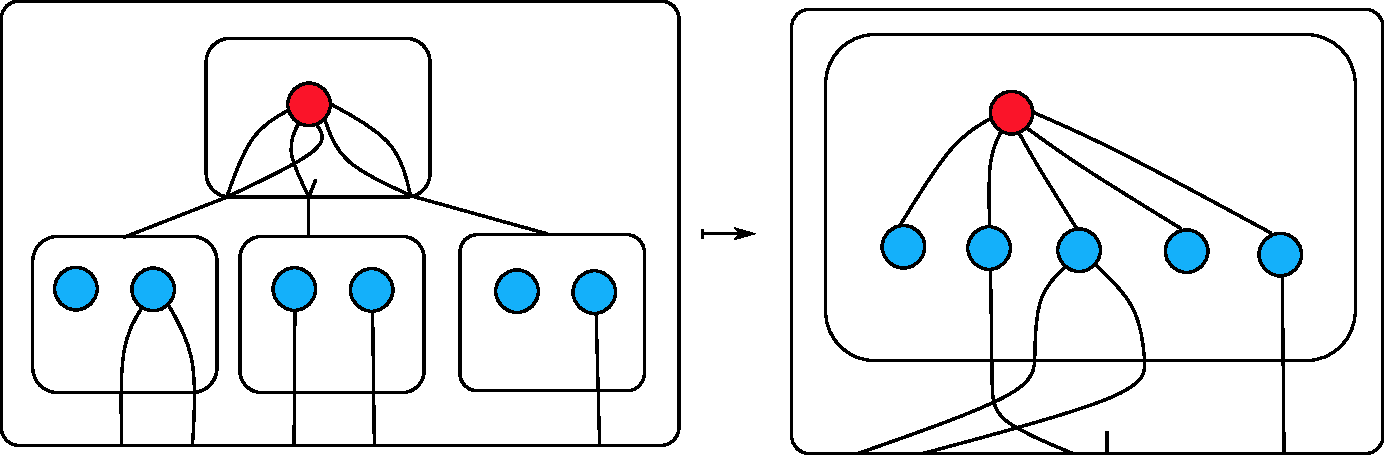
\includegraphics[scale=.35]{pictures/shallow-unfold}
\end{center}
and  defined by
\begin{eqnarray*}
    \xymatrix{
        (a/g)((b_{1,1},\dots,b_{1,k}),\dots, (b_{n,1},\dots,b_{n,k})) 
        % \in  \ranked{\shallowterm  {\reduce k \Gamma} {\Sigma^k}  }
        \ar@{|->}[d]^{\ranked{f_2}} \\
         a(b_{g(1)},\dots,b_{g(m)})/g'
    }
\end{eqnarray*}
where $m$ is the arity of $a$ and the grouping function  $g'$ is  the natural embedding of ports 
% \begin{align*}
% i\in\set{1,\dots,\text{arity of $a$}} \qquad \mapsto  f'(i)=(1, \underset{j<i}{\Sigma} \arity{b_{f(j)}}+1)
% \end{align*}
\begin{align*}
\xymatrix{
    \text{ports of $a(b_{g(1)},\dots,b_{g(m)}))$}
    \ar[d]
    \\
 \displaystyle{\biggl(\coprod_{\substack{i \in \set{1,\ldots,n}\\ j \in \set{1,\ldots,k}}} \text{ports of $b_{i,j}$}, 1 \biggr)} 
}
\end{align*}
\smallskip

\subsubsection{Distribute shallow terms over product}
Finally, consider the function 
\begin{align*}
\ranked{\shallowterm  {\Gamma^k} {\Sigma} \xrightarrow{\quad f_3\quad} (\shallowterm  \Gamma  \Sigma)^k} 
\end{align*}
which distributes shallow terms over the $k$-th power.  This function is illustrated by the following  picture 
\mypic{67}
and defined by 
\begin{eqnarray*}
    \xymatrix{
        (a_1,\dots,a_k)(b_1,\dots,b_n)
        \ar@{|->}[d]^{\ranked{f_2}} \\
        (a_1(b_1,\dots,b_{\text{ar}_1}), a_2(b_{\text{ar}_1+1},\dots,b_{\text{ar}_2}),\dots ,a_k(b_{\text{ar}_{k-1}+1},\dots,b_{\text{ar}_k}))
    }
\end{eqnarray*}
where $\text{ar}_i$ is the arity of $a_i$ for $i\in\set{1,\dots,k}$.

\subsubsection{Unfolding shallow terms.} The following diagram defines  unfolding of shallow terms in terms of the   operations $\ranked{f_1}, \ranked{f_2}, \ranked{f_3}$   defined above:
  \begin{align*}
  \xymatrix@C=2.5cm{
          \ranked{\shallowterm{\mati k \rSigma} {\mati k \rGamma} = {\shallowterm{\reduce k {\Sigma^k}}{\reduce k {\Gamma^k}}} 
        \ar[d]_{\ranked{\substack{f_1}}}
        \ar[r]^-{\ranked{\text{Shallow unfold}}}}
        &
        \ranked{ \reduce k(\shallowterm{\Sigma}{ {\Gamma}})^k = \mati k {(\shallowterm \Sigma \Gamma)}}
        \\
       \ranked{  \reduce k(\shallowterm{\reduce k {\Sigma^k}}{ {\Gamma^k}})}
        \ar[r]_-{\ranked{\flatt\circ \reduce k f_2}}
        &
    \ranked{   \reduce k(\shallowterm{\Sigma^k}{ {\Gamma}}) } \ar[u]^{\ranked{\reduce k  f_3}}
    } 
\end{align*}     

\subsection{Definition of unfolding}
Having defined shallow unfolding, we apply the induction principle described in Section~\ref{sec:terms-induction-principle} to  define unfolding for general terms
\begin{align*}
    \ranked{\unfold : \tmonad \mati k \rSigma \to \mati k {(\tmonad \Sigma)} }.
    \end{align*}
If the input to general unfolding is the identity term $\portletter$, then  the output is:
\mypic{83}
Otherwise, if the input is a nonempty term $a(t_1,\ldots,t_n)$ then the output is obtained by first applying term unfolding to to the smaller terms $t_1,\ldots,t_n$, and then applying the shallow unfold. 